\section{Benchmarking pathway analysis methods}

With description of the characteristics of existing pathway analysis review papers mentioned in the previous section, we propose a comprehensive framework for benchmarking pathway analysis methods that would tackle the limitations and shortcomings of the previous review papers.

Here we introduce two completely objective, reproducible, and scientifically sound approaches to benchmark pathway analysis methods. In the first sub-section, we evaluate the methods based on their ability to identify the involved phenotypes using real human and mouse benchmark data sets. The second sub-section assesses their performances under the true null hypothesis, i.e. there is no true phenotype involved.

\subsection{Systematic assessment of the methods using benchmark data sets}

While some of the review papers discuss the theory aspects of the benchmarking methods or use simulated data sets, very few papers compare the methods using small set of benchmarking data sets with limited number of conditions. 

All   data sets were downloaded from Gene Expression Omnibus database. We normalized them using RMA background adjustment, quantile normalization, and median polish summarization.  We used the \textit{threestep} function from \textit{affyPLM} package to perform those steps. Subsequently, standard genome wide annotation packages corresponding to the platform, e.g. hgu133a.db for HG-U133A, were used to map probes to genes. In case there are multiple probes mapped to the same gene, the median value is chosen.

Six of these are non-TB methods: Fisher's Exact Test \cite{Fisher:1951}, Kolmogorov-Smirnov test \cite{massey1951kolmogorov}, Wilcoxon Rank Sum test \cite{wilcoxon1945individual}, GSA \cite{Efron:2007}, PADOG \cite{Tarca2012down}, and GSEA \cite{Subramanian:2005}. The other five of them are TB methods: SPIA \cite{SPIAversion2.14.0}, ROntoTools \cite{RontoToolsVersion1.2.0}, CePaGSA, CePaORA \cite{gu2012centrality, gu2013cepa}, and PathNet \cite{Dutta:2012}. We provide details of 11 methods that we would do the benchmarking study in Table~\ref{table:PAmethods}. 

\begin{table}

\centering
\caption{Pathway analysis methods investigated in this study. Versions of KEGG of CePa methods are unknown because they are embedded in the software\label{table:PAmethods}} 
\small
\begin{tabular}{@{}clllll@{}}\hline
 & Method & Category  & R-function/package version & Pathway database \\\hline
1 & Fisher's Exact Test &	non-TB 	& fisher.test & KEGG v.65\\ 
2 & WebGestalt &	non-TB 	& WebGestaltR 0.3.1 & KEGG v.65\\ 
3 & GOstats &	non-TB 	&2.48.0 & KEGG v.65\\ 
4 & Kolmogorov-Smirnov Test& non-TB & ks.test & KEGG v.65\\
5 & Wilcoxon rank sum	& non-TB 	& wilcox.test &  KEGG v.65\\
6 & GSEA &	non-TB & 1.0 & KEGG v.65\\
7 & GSA &	non-TB & 1.03 & KEGG v.65\\
8 & PADOG &	non-TB & 1.20.0 & KEGG v.65\\
9 & SPIA &	TB  & 2.30.0 & KEGG v.65\\
10 & ROntoTools &		TB & 2.6.0 & KEGG v.65\\
11 & CePaORA &	TB & 0.5 & KEGG (version unknown)\\
12 & CePaGSA &	TB & 0.5 & KEGG (version unknown)\\
13 & PathNet &	TB & 1.18.0 & KEGG v.56\\
\hline
\multicolumn{5}{l}{\textit{non-TB}: non topology-based method, \textit{TB}: topology-based method}

\end{tabular}
\end{table}


\subsubsection{Ability to identify the target pathways on human data sets}

One of the most straightforward ways of validating a pathway analysis method is assessing its ability to identify the target pathway describing the related mechanism of the condition studied. 
This validation approach works as follows. First, data sets related to  conditions that already have an associated KEGG pathway (i.e. target pathway) are collected. For each experiment, a perfect method would be able to identify the target pathway as significantly impacted and rank it on top. The target pathway is chosen in advance without human interpretation. Hence, this validation is completely objective and scientifically sound. We apply each method on each of those data sets and report the ranks and p value of target pathways (Fig \ref{workflow}).

\begin{figure}
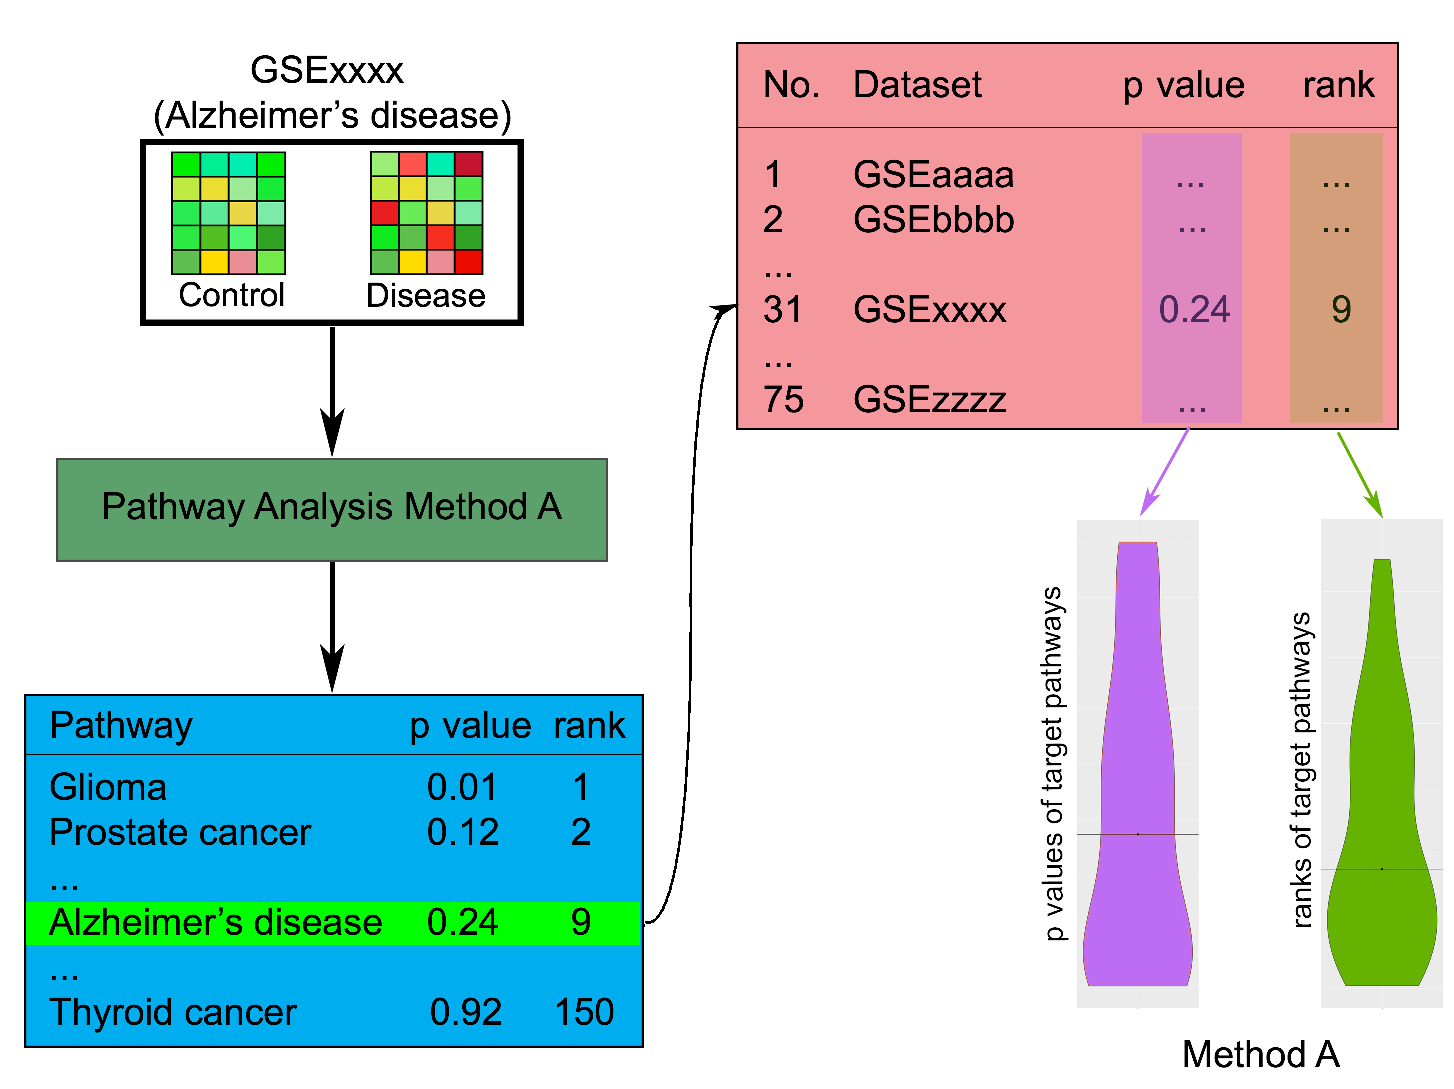
\includegraphics[width=0.8\linewidth]{Figures/Fig1}
\caption{\textbf{The process of evaluating a pathway analysis method based on their ability to identify target pathways.} Each pathway analysis method is applied on 75 data sets. Methods are evaluated based on their ability to rank the target pathways. In this example, a data set of Alzheimer's disease is examined, and thus the target pathway is ``Alzheimer's disease". Each method produces lists of ranks and p value of the target pathways, which are then used to assess its performance.}
\label{workflow}
\end{figure}

Here, we propose using 75 human data sets and 11 mouse data sets for the comparison. We also take the bias of the methods towards some conditions into consideration. To make it even fairer competition, we choose the same number of data sets per conditions. In fact, we choose 15 widely studied conditions, and 5 data sets per conditions.

Table \ref{table:HumanDatasets} provides detailed information regarding the 75 human data sets used for benchmarking methods' ability to identify target pathways. This information includes: GEO ID, disease, number of normal samples and phenotype samples,  Pubmed ID, tissue from which the samples were taken, and the platform used for the experiment.

\begin{landscape}
\setlength\LTleft{0pt}            % default: \parindent
\setlength\LTright{0pt}           % default: \fill

\centering
\small
\begin{longtable}{lp{4cm}cccp{4cm}l}
\caption{75 benchmark data sets of 15 diseases used to compare 11 methods in this paper.}\\
\hline
 \textbf{GEO ID}& \textbf{Disease/Condition} & \textbf{\#Normal} & \textbf{\#Condition} & \textbf{Pubmed ID} & \textbf{Tissue} & \textbf{Platform}  \\
 \hline
GSE781 & Renal cell carcinoma	& 5	& 12	& 14641932 &	Kidney &	HG-U133A \\
GSE14762	&Renal cell carcinoma	&12	&9	&19252501	&Kidney	&HG-U133Plus 2.0 \\
GSE6357	&Renal cell carcinoma	&12	&6	&27063186	&CD8+ T Cell	&HG-U133A\\
GSE6344	&Renal cell carcinoma	&10	&10	&17699851	&Clear cell RCC	&HG-U133A\\
GSE48352	&Renal cell carcinoma	&8	&24	&NA	&Kidney	&HG-U133Plus 2.0\\
GSE1297	&Alzheimer’s disease	&9	&7	&14769913	&Hippocampal CA1	&HG-U133A\\
GSE5281EC	&Alzheimer’s disease	&13	&10	&17077275	&Brain, Entorhinal Cortex	& HG-U133Plus 2.0\\
GSE5281HIP	&Alzheimer’s disease	&13	&10	&17077275	&Brain, hippocampus	& HG-U133Plus 2.0\\
GSE5281VCX&	Alzheimer’s disease	&12	&19	&17077275	&Brain, primary visual cortex	& HG-U133Plus 2.0\\
GSE16759	&Alzheimer’s disease&	8	&4	&20126538	&Parietal lobe	&HG-U133Plus 2.0\\
GSE3467&	Thyroid cancer	&9	&9	&16365291	&Thyroid	&HG-U133Plus 2.0\\
GSE3678	&Thyroid cancer	&7	&7	&NA	&Thyroid	&HG-U133Plus 2.0\\
GSE58545	&Thyroid cancer	&18	&27	&26625260	&Thyroid	&HG-U133A\\
GSE85457	&Thyroid cancer	&3	&4	&NA	&Thyroid	&HG-U133Plus 2.0\\
GSE58689	&Thyroid cancer	&18	&27	&26625260	&Thyroid	&HG-U133A\\
GSE3585	&Dilated cardiomyopathy	&5	&7	&17045896	&Heart, subendocardial left ventricular	&HG-U133A\\
GSE33970	&Dilated cardiomyopathy	&18	&5	&NA	&Whole blood and heart	&HG-U133Plus 2.0\\
GSE29819	&Dilated cardiomyopathy	&12	&14	&22085907	&Heart, left and right ventricular	&HG-U133Plus 2.0\\
GSE79962	&Dilated cardiomyopathy	&11	&9	&NA	&Heart	&HuGene-10st\\
GSE21610	&Dilated cardiomyopathy	&8	&42	&20460602	&Heart	&HG-U133Plus 2.0\\
GSE4107	&Colorectal cancer	&10	&12	&17317818	&Colonic mucosa	&HG-U133Plus 2.0\\
GSE8671	&Colorectal cancer	&32	&32	&18171984	&Colon	&HG-U133Plus 2.0\\
GSE9348	&Colorectal cancer	&12	&70	&20143136	&Colon	&HG-U133Plus 2.0\\
GSE23878	&Colorectal cancer	&19	&19	&21281787	&Colon	&HG-U133Plus 2.0\\
GSE4183	&Colorectal cancer	&8	&15	&18776587	&Colon	&HG-U133Plus 2.0\\
GSE6956C	&Prostate cancer	&11	&36	&18245496	&Prostate	&HG-U133A 2\\
GSE6956AA	&Prostate cancer	&7	&33	&18245496	&Prostate	&HG-U133A 2\\
GSE55945	&Prostate cancer	&7	&12	&19737960	&Prostate	&HG-U133Plus 2.0\\
GSE26910	&Prostate cancer	&6	&6	&21611158	&Prostate	&HG-U133Plus 2.0\\
GSE104749	&Prostate cancer	&4	&4	&NA	&Prostate	&HG-U133Plus 2.0\\
GSE8762	&Huntington’s disease	&10	&12	&17724341	&Lymphocyte	&HG-U133Plus 2.0\\
GSE24250	&Huntington’s disease	&6	&8	&21969577	&Venous cellular whole blood	&HG-U133A\\
GSE73655	&Huntington’s disease	&7	&13	&26756592	&Subcutaneous adipose	&HuGene-10st\\
GSE45516	&Huntington’s disease	&3	&6	&24296361	&Fibroblasts	&HG-U133Plus 2.0\\
GSE37517	&Huntington’s disease	&5	&8	&22748968	&Neural stem cell	&HuGene-10st\\
GSE9476	&Acute Myeloid Leukemia	&37	&26	&17910043	&Peripheral blood, bone marrow	&HG-U133A\\
GSE14924\_CD4	&Acute Myeloid Leukemia&	10	&10	&19710498	&CD4 T Cell	&HG-U133Plus 2.0\\
GSE14924\_CD8	&Acute Myeloid Leukemia		&11	&10	&19710498	&CD8 T Cell	&HG-U133Plus 2.0\\
GSE92778	&Acute Myeloid Leukemia	&6	&6	&29035359	&Bone marrow stroma cells	&HuGene-10st\\
GSE68172	&Acute Myeloid Leukemia	&5	&72	&NA	&LSC, HSC and leukemic bulk AML \textsuperscript{*}	&HG-U133Plus 2.0\\
GSE15471	&Pancreatic cancer	&35	&35	&19260470	&Pancreas	&HG-U133Plus 2.0\\
GSE16515	&Pancreatic cancer	&15	&15	&19732725	&Pancreas	&HG-U133Plus 2.0\\
GSE32676	&Pancreatic cancer	&7	&25	&22261810	&Pancreas		&HG-U133Plus 2.0\\
GSE28735	&Pancreatic cancer	&45	&45	&23918603	&Pancreas		&HuGene-10st\\
GSE18670	&Pancreatic cancer	&6	&18	&23157946	&Pancreas	&HG-U133Plus 2.0\\
GSE18842	&Non-small cell lung cancer	&44	&44	&20878980	&Lung	&HG-U133Plus 2.0\\
GSE19188	&Non-small cell lung cancer	&62	&91	&20421987	&Lung	&HG-U133Plus 2.0\\
GSE19804	&Non-small cell lung cancer	&60	&60&	20802022	&Lung	&HG-U133Plus 2.0\\
GSE50627	&Non-small cell lung cancer	&6	&9	&25881239	&Lung	&HuGene-10st\\
GSE6044	&Non-small cell lung cancer	&5	&31	&18992152	&Lung	&HG-Focus\\
GSE19728	&Glioma	&4	&17	&21836821	&Brain	&HG-U133Plus 2.0\\
GSE21354	&Glioma	&4	&13	&21836821	&Brain	&HG-U133Plus 2.0\\
GSE50161	&Glioma	&13	&95	&24078694	&Brain	&HG-U133Plus 2.0\\
GSE4290	&Glioma	&23	&157	 & 16616334	&Brain	&HG-U133Plus 2.0\\
GSE44971	&Glioma	&9	&49	&23660940	&Brain	&HG-U133Plus 2.0\\
GSE20153	&Parkinson’s disease	&8	&8	&20926834	&B lymphocytes from peripheral blood	&HG-U133Plus 2.0\\
GSE20291	&Parkinson’s disease	&20	&15	&15965975	&Brain	&HG-U133A\\
GSE20164	&Parkinson’s disease	&5	&6	&20926834	&Substantia nigra (midbrain)	&HG-U133A\\
GSE7621	&Parkinson’s disease	&9	&16	&17571925	&Substantia nigra (midbrain)	&HG-U133Plus 2.0\\
GSE19587	&Parkinson’s disease	&10	&12	&20837543	&Brain	&HG-U133A 2\\
GSE19420	&Type II diabetes mellitus	&12	&12	&22802091	&Skeletal muscle vastus lateralis	&HG-U133Plus 2.0\\
GSE39825	&Type II diabetes mellitus	&6	&4	&23919306	&Fibroblasts (cell culture)	&HG\_U95Av2\\
GSE26887	&Type II diabetes mellitus	&5	&7	&22427379	&Left ventricle	&HuGene-10st\\
GSE21340	&Type II diabetes mellitus	&15	&5	&23919306	&Skeletal muscle	&HG\_U95Av2\\
GSE38642	&Type II diabetes mellitus	&54	&9	&22768844	&Pancreatic islets	&HuGene-10st\\
GSE24739\_G0	&Chronic Myeloid Leukemia	&4	&8	&21436996	&Peripheral blood	&HG-U133Plus 2.0\\

GSE24739\_G1	&Chronic Myeloid Leukemia	&4	&8	&21436996	&Peripheral blood	&HG-U133Plus 2.0 \\
GSE33075	&Chronic Myeloid Leukemia	&18	&9	&22388797	&Bone marrow	&HG-U133Plus 2.0 \\
GSE24739	&Chronic Myeloid Leukemia	&8	&16	&21436996	&Peripheral blood and bone marrow	&HG-U133Plus 2.0\\
GSE1418	&Chronic Myeloid Leukemia	&6	&8	&15618956	&Bone marrow	&HG-Focus\\
GSE7305	&Endometrial cancer	&10	&10	&17640886	&Endometrium/Ovarian tissue	&HG-U133Plus 2.0\\
GSE63678	&Endometrial cancer	&5	&7	&26559525	&Endometrium	&HG-U133A\\
GSE7803	&Endometrial cancer	&10	&31	&17974957	&Cervix and squamous cervical epitheilium	&HG-U133A\\
GSE17025	&Endometrial cancer	&12	&91	&21619611	&Endometrium	&HG-U133Plus 2.0\\
GSE36389	&Endometrial cancer	&7	&13	&NA	&Endometrium	&HG-U133A\\
\hline
\multicolumn{7}{l}{\textsuperscript{*}\footnotesize{Leukemic stem cells (LSC), hematopoietic stem cells (HSCs), and AML bulk cells (CD34+CD38+, CD34-CD38+ and CD34-CD38)}}
\label{table:HumanDatasets}
\end{longtable}
\end{landscape}


%Among the widely used methods described in the previous section, we would choose eleven methods in each groups to perform on real 75 data sets to prepare their individual performances. 

\subsubsection{Ability to identify the pathways containing the cause of the phenotype on mouse data sets}
\label{KOsubsubsection}

Although the above assessment is better than the human interpretation approach or using simulated data sets, it still has some limitations: it focuses solely on one true positive, the target pathway. We do not know what other pathways are also truly impacted and therefore cannot evaluate other criteria such as the accuracy, specificity, sensitivity, and the AUC of a method. Here, we use knock-out data sets that involve using knock-out experiments (KO), where the source of the perturbation is known, i.e. the KO gene.

Table \ref{table:MouseDatasets} provides detailed information regarding the 11 benchmark KO data sets used. This information includes:  the GEO ID, symbol of KO gene, number of truly impacted pathways, number of normal samples, number of phenotype samples, Pubmed ID, tissue from which the samples were taken, and the platform used for the experiment.


We consider pathways containing the KO gene as positives and the others as negatives. After performing the pathway analysis method on this data set, a p value threshold of 0.05 is used to determine whether a pathway is significantly impacted. A true positive (TP) is a positive which is correctly identified as significant. 
Similarly, a true negative (TN) is a negative which is correctly identified as insignificant.
A false positive (FP) is a pathway that does not contain the KO gene but is reported as significant. A false negative (FN) is a pathway that contains the KO gene but is not reported as significant.
Subsequently, we calculate the accuracy, sensitivity, specificity, and AUC of methods studied using 11 KO data sets. 
We also perform a higher level comparison between the ranks and p value of the target pathways obtained by non-TB and TB methods.


\begin{landscape}
\setlength\LTleft{0pt}            % default: \parindent
\setlength\LTright{0pt}           % default: \fill
\centering
\small
\begin{longtable}{@{}llccccll@{}}
\caption{Eleven knockout benchmark data sets used to compare 10 methods in this paper.\label{table:MouseDatasets}}\\
\hline
 \textbf{GEO ID}& \textbf{KO gene} & \makecell{\textbf{\#Impacted} \\\textbf{Pathways} }& \textbf{\#Nornal} & \textbf{\#Condition}& \textbf{Pubmed ID} & \textbf{Tissue} & \textbf{Platform}  \\
 \hline
GSE22873	&Myd88	&19	&11	&8	&22075646	&Liver				&Mouse430\_2 \\
GSE6030		&Neurod1	&1	&3	&3	&17630985	&Pineal gland			&Mouse430\_2 \\
GSE29048	&Pdx1	&3	&4	&4	&22135308	&Intestinal epithelium	&Mouse430\_2\\
GSE70302	&IL1a	&20	&4	&4	&26224856	&Spinal cord			&MoGene-1\_0-st\\
GSE70302	&IL1b	&34	&4	&4	&26224856	&Spinal cord			&MoGene-1\_0-st\\
GSE58120	&IL2		&3	&6	&6	&25652593	&Myeloid dendritic cells	&MoGene-1\_0-st\\
GSE46211	&TGFBR2	&20	&12	&6	&24496627	&Anterior \& posterior palatal tissue	&Mouse430\_2\\
GSE49166     &BHLHE40	&1	&3	&3	&24699451	&CD4 T cells			&MoGene-1\_0-st\\
GSE50933	&ID3		&2	&5	&5	&24244015	&Natural killer T cells	&Mouse430\_2\\
GSE62999	&DUSP5	&1	&10	&10	&25398911	&Bone marrow			&Mouse430\_2\\
GSE57917    &ONECUR1	&2	&3	&3	&25313862	&Retinas				&Mouse430\_2\\
\hline
 \end{longtable}
\end{landscape}

\subsection{Investigation of the bias under the null}

In this benchmark, we conduct a deeper investigation into the behavior of these methods under the null hypothesis. 
Here, we create a true null hypothesis by using simulated data sets that are constructed by randomly selected healthy samples from the 75 aforementioned data sets.
We apply each method  more than 2,000 times, each time on different simulated data sets.
Each pathway then has an empirical null distribution of p values resulting from those 2,000 runs (Fig \ref{nullGeneration}).
When the null hypothesis is true, p value obtained from any sound statistical test should be uniformly distributed  between 0 and 1 \cite{barton2013correction, fodor2007towards}.
However, p value generated from many pathway analysis methods are often unimodal (biased toward 0 or 1) or bimodal (biased toward 0 and 1) (Fig. \ref{fig:Biased0} and Fig. \ref{fig:Biased1}). 

\begin{figure}
\centering
%  \captionsetup{width=.8\linewidth}

	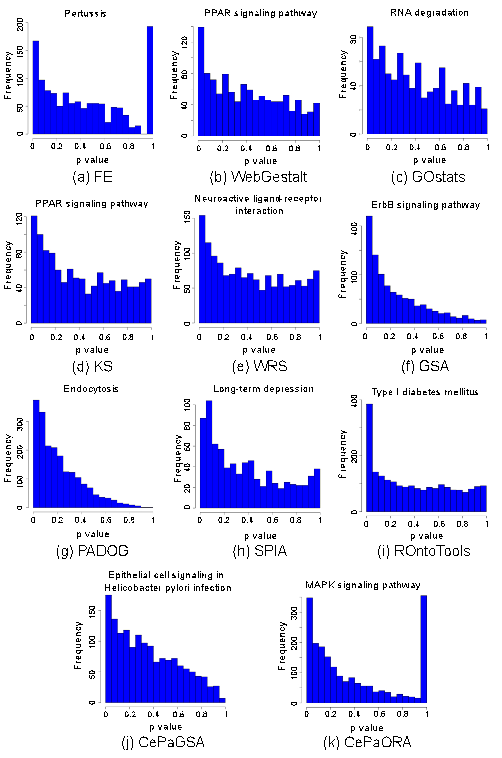
\includegraphics[width=0.8\linewidth]{Figures/Biased0}
	\caption{\textbf{Examples of pathways that have empirical null distributions of p values biased toward 0.} The procedure for generating null distributions is described in Fig. \ref{nullGeneration}. The x-axes display the p values whereas the y-axes display the frequencies. These pathways are likely to be falsely identified as significantly impacted by the corresponding method (false positive).}\label{fig:Biased0}
\end{figure}

\begin{figure}
\centering
%  \captionsetup{width=.8\linewidth}

	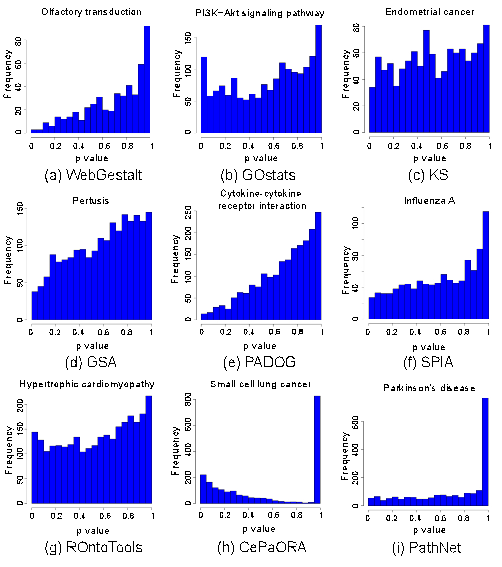
\includegraphics[width=1\linewidth]{Figures/Biased1}
	\caption{\textbf{Examples of pathways that have empirical null distributions of p values biased toward 1.} In these sub-figures, x-axes represent the p value, while y-axes represent their frequencies. These pathways are often incorrectly excluded in the list of significant pathways  by the corresponding method even when they are indeed impacted (false negative).}\label{fig:Biased1}
\end{figure}


More specifically, a null distribution of p value of a pathway generated by a method skewed to the right (biased toward 0) shows that this method has a tendency to yield low p value and therefore report the pathway as significantly impacted even when it is not (false positive). By contrast, a null distribution of p value of a pathway skewed to the left (biased toward 1) indicates that the given method tends to produce consistently higher p value thus possibly report this pathway as insignificant when it is indeed impacted (false negative).
The results of this null-hypothesis analysis may explain why some methods work well for certain diseases while they perform poorly for others. If a method is biased to report more often a given cancer pathway as significant, that method may be perceived to perform better in experiments involving that particular type of cancer. 

\begin{figure}
\centering
	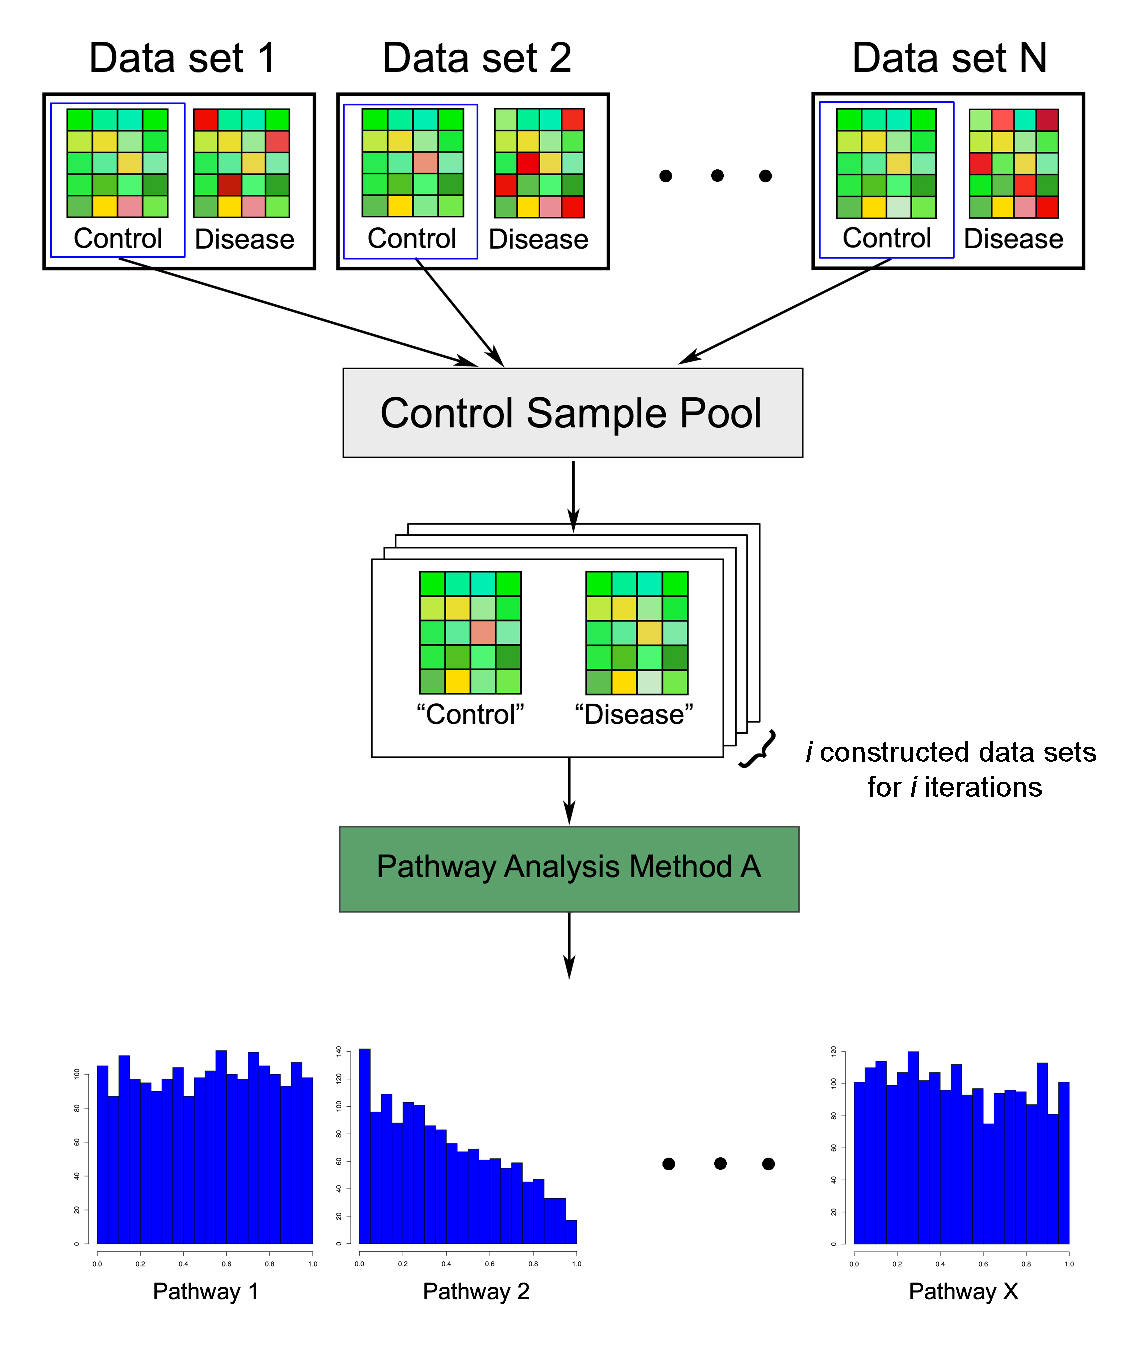
\includegraphics[width=0.8\linewidth]{Figures/Fig4}
  \caption{\textbf{The process of creating the null distributions of p value for all pathways by a given pathway analysis method.} Control samples from data sets are  gathered to construct a control sample pool. To create the null distribution of p value of all pathways under the null for each method, more than 2,000 iterations were performed. The data sets used in these iterations are generated by randomly selecting samples from the control sample pool.}
  \label{nullGeneration}
\end{figure}

We would also report the total number of biased pathways  (either toward 0 or 1) produced by these methods.
%The number of biased pathways is at least 66 for all the methods compared in this work, except GSEA which has no biased pathway was found. 
%While investigating more, we found that the aggregate p value of all the pathways generated by GSEA is uniformly distributed under the null (Additional file 1: Fig. \ref{fig:GSEAagg}).
%A similar conclusion about GSEA was also reached by Nguyen \textit{et al.}~\cite{nguyen2017DANUBE}.

%The number of pathways biased toward 0 produced by 13 methods are shown in Figure \ref{fig:NumberOfBias}b.
%The figure shows that performing pathway analysis using FE test produces the highest number (137 out of 150 pathways) of false positives, this is followed by WRS test (114 out of 150 pathways) and CePaGSA (112 out of 186 pathways). On the other hand, GSEA and PathNet produce no false positive pathways.
%
%Similarly, the numbers of pathways biased toward 1 produced by different methods are shown in Figure \ref{fig:NumberOfBias}c.
%PathNet produces the highest number (129 out of 130 pathways) of false negative pathways.
%No false negative pathways are identified while performing pathway analysis using GSEA, CePaGSA, WRS test and FE test.

%\begin{figure}[!h]
%	\includegraphics[width=0.7\linewidth]{picturesForGB/NrBiasedPathway}
%        \caption{\csentence{The number of biased pathways calculated based on Pearson's moment coefficient.}  Under the true null hypothesis, an ideal method would produce a uniform distribution of p value from 0 to 1 for every pathway. Here, thresholds of Pearson's moment coefficient of $0.1$ and $-0.1$ are used to determine if the empirical distribution p values is biased toward 0 or 1, respectively.
%        Panel (a) shows the total number of biased  pathways (toward either 0 or 1) produced by each method.
%Each method, except GSEA, has at least 66 biased pathways.
%Panel (b) shows the number of pathways biased toward 0 (false positives) produced by different methods.
%FE  produces the highest number (137 out of 150 pathways) of false positives, followed by WRS  (114 out of 150) and CePaGSA (112 out of 186).
%Panel (c) shows the number of pathways biased toward 1 (false negatives) produced by different methods.
%PathNet produces the highest number (129 out of 130) of false negative pathways. The methods in red are TB methods. The methods in blue are non-TB methods}\label{fig:NumberOfBias}
%\end{figure}


%\begin{figure}[h]
%	\includegraphics[width=0.8\linewidth]{picturesForGB/NrMethodsBiased}
%
%        \caption{\csentence{The number of methods biased for each pathway.} The y-axis shows the KEGG pathways, while the x-axis indicates the number of methods biased toward 0 and  1, respectively. Each horizontal line represents a pathway. The lengths of the blue and red lines show the number of methods in this study biased toward 0 and 1, respectively. Pathways are sorted by the number of methods biased. There is no pathway that is unbiased for all methods. The top 10 least and top 10 most biased pathways are shown by name.}\label{fig:PathwaysDist}
%\end{figure}



